%
% capitulo Introduccion
%
\chapter{Introducci\'{o}n}

%
% defincion matematica de los Majorana 
%
\section{Definici\'{o}n}
Los llamados modos de Majorana fueron inicialmente planteados por Etore Majorana \cite{Majorana1937TeoriaSD}. Estos los defini\'{o} de tal forma que la part\'{i}cula sea la misma que la antipart\'{i}cula. En t\'{e}rminos de operadores de segunda cuantizaci\'{o}n tienen la propiedad 
\begin{equation}
    \gamma^\dagger=\gamma
\end{equation}
Asimismo, estos obedecen las siguientes reglas de anticonmutaci\'{o}n
\begin{equation}
    \{\gamma_i,\gamma_j\}=2\delta_{ij}
\end{equation}
Todo modo de Majorana puede ser definido en t\'{e}rminos de operadores fermi\'{o}nicos
\begin{equation}
    \gamma=c+c^\dagger
\end{equation}
De igual manera, un modo fermi\'{o}nico ordinario $c^\dagger$ puede ser definido en t\'{e}rminos de dos modos de Majorana como:
\begin{equation}
    c^\dagger=\frac{1}{2}(\gamma_1-i\gamma_2)
\end{equation}

Hasta hora solo hemos hecho una definici\'{o}n matem\'{a}tica pero lo que nos importa es su uso en la f\'{i}sica.

En f\'{i}sica de altas energ\'{i}as los fermiones de Majorana todav\'{i}a no han sido hallados, aunque todav\'{i}a queda por ver si los neutrinos clasifican como estos. En materia condensada, por otra parte, los buscamos como quasipart\'{i}culas. Las b\'{u}squeda de Majoranas se volvi\'{o} una l\'{i}nea de investigaci\'{o}n importante por su posible uso en computaci\'{o}n cu\'{a}ntica. 

Si tenemos una cadena con varios sitios fermi\'{o}nicos numerados $1,...,N$, en modos de Majorana los sitios podr\'{i}an ser escritos como 
\begin{equation}
    \begin{split}
        c_1&=\frac{1}{2}(\gamma_1+i\gamma_2),\quad c^\dagger_1=\frac{1}{2}(\gamma_1-i\gamma_2)\\
        c_2&=\frac{1}{2}(\gamma_3+i\gamma_4),\quad c^\dagger_2=\frac{1}{2}(\gamma_3-i\gamma_4)\\
        &.\\
        &.\\
        &.\\
        c_N&=\frac{1}{2}(\gamma_{2N-1}+i\gamma_{2N}),\quad c^\dagger_2=\frac{1}{2}(\gamma_{2N-1}-i\gamma_{2N})
    \end{split}
\end{equation}
Ya que siempre podemos expresar un fermi\'{o}n como dos modos de Majorana, en principio un Hamiltoniano tambi\'{e}n puede ser enteramente descrito por ellos. Hasta ahora no hemos hecho m\'{a}s que definir los Majorana en relaci\'{o}n con los fermiones pero pronto se les dar\'{a} un significado a un Majorana individual.
%
%
%
\section{Aniones}
Los modos de Majorana no pueden ser identificados ni como fermiones ordinarios ni como bosones, la estad\'{i}stica que presentan u obedecen es diferente. En el caso de las part\'{i}culas indistingibles, que acabamos de mencionar, al ser intercambiadas adquieren o no un cambio de signo en la funci\'{o}n de onda. 
\begin{equation}
\begin{split}    \psi(x_1,x_2)&=+\psi(x_2,x_1)\rightarrow\text{Bosones}\\
    \psi(x_1,x_2)&=-\psi(x_2,x_1)\rightarrow\text{Fermiones}
\end{split}
\end{equation}
Podemos pensar en este cambio de signo como un cambio de fase que la funci\'{o}n de onda adquiere cuando f\'{i}sicamente movemos las part\'{i}culas alrededor una de la otra. Pensar en esto en una sola dimensi\'{o}n puede no tener sentido ya que no habr\'{i}a espacio para el intercambio. Sin embargo, en dos dimensiones se encuentra una nueva forma de pensar en la fase adquirida por las funciones de onda. 

Supongamos que tenemos dos part\'{i}culas id\'{e}nticas en dos dimensiones y las intercambiamos de la forma que hemos descrito, o sea movi\'{e}ndolas una alrededor de la otra. La funci\'{o}n de onda adquirir\'{a} una fase. La forma en c\'{o}mo las moveremos ser\'{a} en sentido antihorario. 
\begin{equation}
    \psi(x_1,x_2)\rightarrow e^{i\theta}\psi(x_1,x_2)
\end{equation}
Si realizamos de nuevo el intercambio en sentido antihorario, la nueva fase no ser\'{a} $+$ o $-$, sino una fase no trivial $e^{i2\theta}$.
\begin{equation}
    \psi(x_1,x_2)\rightarrow e^{i2\theta}\psi(x_1,x_2)
\end{equation}
El caso especial de $\theta=0,\pi$ pertenece al de los bosones y fermiones, respectivamente. Esto quiere decir que existe todo un espectro de estad\'{i}sticas $\theta$ y cuyas part\'{i}culas que la obedecen las llamaremos \emph{aniones}. Esta estad\'{i}stica tambi\'{e}n es llamada \emph{estad\'{i}stica fraccionaria}. La idea de los aniones fue explorada primero por Frank Wikczek\cite{PhysRevLett49957}\cite{RevModPhys801083}.\\
A partir de estas ideas se puede hablar de operaciones de trenzado (\emph{braiding operations}) en las que una operaci\'{o}n del grupo de trenzas (\emph{braid group}) puede ser visualizado como un conjunto de trayectorias de las part\'{i}culas en la dimensi\'{o}n $2+1$ espacio-tiempo en el que las dos part\'{i}culas se cruzan pero de tal forma que podamos diferenciar el camino que tom\'{o} cada una.
Por ejemplo $\sigma_1$ y $\sigma_2$ vendr\'{i}an a ser estas operaciones del grupo de trenzado tal que las part\'{i}culas afectadas tendr\'{a}n que seguir las trayectorias como en la figura\ref{fig:braiding}. El saber qu\'{e} trayectoria est\'{a} por encima de otra es importante porque no es lo mismo aplicar $\sigma_1\sigma_2$ que $\sigma_2\sigma_1$, es decir el grupo de trenzado es un \emph{grupo no-abeliano}. 
%
% Operaciones de Braiding
%
\begin{figure}[H]
    \centering
    \includegraphics[width=0.80\textwidth]{ch1f/braiding.png}
    \caption{Aplicaci\'{o}n de operaciones de trenzado. En todos los casos presentes se consideran tres part\'{i}culas las cuales poseen trayectorias que las vamos a ir modificando dependiendo de qu\'{e} operaci\'{o}n de trenzado aplicamos. Si las posiciones en las que terminan las part\'{i}culas son las mismas en las que empezaron sin importar las operaciones que se aplicaron entonces estas ser\'{a}n equivalentes.}
    \label{fig:braiding}
\end{figure}
La raz\'{o}n porque nos interesan los modos de Majorana y la estad\'{i}stica no-abeliana dada es porque una forma de atacar el problema de las computadoras cu\'{a}nticas tolerantes a fallos \cite{KITAEV20032}\cite{Bravyi2000FermionicQC} es embeber informaci\'{o}n de forma robusta en fermiones no locales, los cuales pueden encontrarse como quasipart\'{i}culas con el comportamiento de aniones, m\'{a}s espec\'{i}ficamente Majoranas.\\
Ahora imaginemos que tenemos a cuatro Majoranas en un cable unidimensional, si quisieramos intercambiarlos de posici\'{o}n inevitablemente estos se encontrar\'{i}an y colisionan, por esta raz\'{o}n la estad\'{i}stica no est\'{a} bien definida para esta dimension. Para realizar operaciones con fermiones de Majorana necesitamos tenerlos siempre distanciados y es ah\'{i} donde entra el concepto de \emph{braiding}, que pict\'{o}ricamente se puede ver como una uni\'{o}n o empalme al superconductor unidimensional donde podemos guardar a un Majorana (rojo) como en la figura \ref{fig:braiding1} y podemos ahora pasar el Majorana (azul) de la derecha a la izquierda, y, asimismo pasar el Majorana guardado (rojo) a la derecha como en la figura \ref{fig:braiding2}. En mec\'{a}nica cu\'{a}ntica operaciones como estas usualmente se escriben como una transformaci\'{o}n $\ket\Psi\rightarrow U\ket\Psi$, en el caso de fermiones o bosones el $U$ es una constante $+1$ o $-1$ seg\'{u}n corresponde. Bajo las condiciones que nos imponen los Majoranas es enteramente posible que $U$ sea otra cosa que $\pm 1$, sino que puede llegar a ser una matriz de rotati\'{o}n que aplicamos a la funci\'{o}n de onda. Si tenemos varias operaciones de \emph{braiding} o simplemente intercambio significa que aplicaremos varias rotaciones, es decir, multiplicaci\'{o}n de matrices y estas operaciones pueden ser no-conmutativas.
\begin{figure}[ht]
\centering
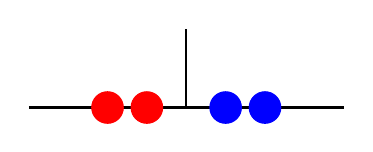
\begin{tikzpicture}
    % Horizontal line
    \draw[thick] (0,0) -- (4,0);
    % Vertical line in the middle (T shape)
    \draw[thick] (2,0) -- (2,1);
    % Red balls on the left
    \filldraw [red] (1,0) circle (0.2);
    \filldraw [red] (1.5,0) circle (0.2);
    % Blue balls on the right
    \filldraw [blue] (2.5,0) circle (0.2);
    \filldraw [blue] (3,0) circle (0.2);
\end{tikzpicture}
\caption{Se tiene la esperanza de que con los modos de Majorana ser\'{a} posible hacer operaciones l\'{o}gicas con qubits, este dibujo rudimentariamente presenta una operaci\'{o}n simple que es la de intercambiar de lugar a dos Majoranas.}
\label{fig:braiding1}
\end{figure}

\begin{figure}[ht]
\centering
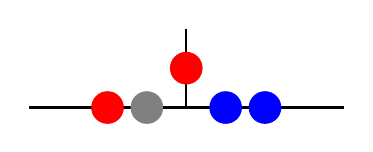
\begin{tikzpicture}
    % Horizontal line
    \draw[thick] (0,0) -- (4,0);
    % Vertical line in the middle (T shape)
    \draw[thick] (2,0) -- (2,1);
    % Red ball on the vertical line
    \filldraw [red] (2,0.5) circle (0.2);
    % Other red ball on the left
    \filldraw [red] (1,0) circle (0.2);
    \filldraw [gray] (1.5,0) circle (0.2);
    % Blue balls on the right
    \filldraw [blue] (2.5,0) circle (0.2);
    \filldraw [blue] (3,0) circle (0.2);
\end{tikzpicture}
\caption{Ya que tener cable unidimensional no permitir\'{i}a el intercambio, si hacemos un acople al cable con alguna otra juntura donde podamos almacenar momentaneamente a uno de los Majorana entonces ah\'{i} s\'{i} es posible llevar a cabo la operaci\'{o}n.}
\label{fig:braiding2}
\end{figure}
La raz\'{o}n porque nos interesan los modos de Majorana y la estad\'{i}stica no-abeliana dada es porque una forma de atacar el problema de las computadoras cu\'{a}nticas tolerantes a fallos \cite{KITAEV20032}\cite{Bravyi2000FermionicQC} es embeber informaci\'{o}n de forma robusta en fermiones no locales, los cuales pueden encontrarse como quasipart\'{i}culas con el comportamiento de aniones, m\'{a}s espec\'{i}ficamente Majoranas. Una vez que tenemos Majoranas queremos realizar operaciones sobre qubits, pero, como hemos visto, esto se puede lograr usando operaciones de trenzado.\\
Por otro lado, hablar de aniones no solo nos limita al campo de materia condensada. El tema nos conecta directamente con el estudio de computaci\'{o}n cu\'{a}ntica topol\'{o}gica \cite{freedman2000} y teor\'{i}a cu\'{a}ntica de campos topol\'{o}gica \cite{lancaster2014quantum}\cite{ZeeQuantum} que, otra vez, nos vuelve a conectar con temas de materia condensada como por ejemplo: el estudio de v\'{o}rtices, el efecto Aharonov-Bohm o la teor\'{i}a de Chern-Simons \cite{Witten}.\\
Desde el 2021, luego de bastantes a\~{n}os de resultados parciales en la b\'{u}squeda de Majoranas, combinando t\'{e}cnicas te\'{o}ricas y experimentales de BEC (condensado de Bose-Einstein) y BCS (teor\'{i}a de superconductividad de Bardeen–Cooper–Schrieffer) \cite{anyonsandmajo} hay mucha promesa en por fin poder identificar aniones, en particular Majoranas.
\section{Introducci\'{o}n a la cadena de Kitaev}
Debido a su relevancia para nuestros resultados novedosos con la cadena de Kitaev interactuando con un punto cu\'{a}ntico, repasamos brevemente la cadena aislada.

En resumen, el paper de Kitaev \cite{YKitaev_2001} nos cuenta que en un sistema fermi\'{o}nico sin esp\'{i}n con una brecha en el espectro del volumen posee estados de borde que pueden ser descritos por fermiones de Majorana, que podr\'{i}an ser de utilidad como qubits por ser robustos ante perturbaciones.

El sistema fermi\'{o}nico que nos plantea Kitaev es el de una cadena unidimensional en el r\'{e}gimen sin esp\'{i}n (esto se podr\'{i}a lograr aplicando un campo magn\'{e}tico), superconductor (por superconductividad inducida por proximidad) en el que exista una brecha en el espectro. Con esta receta podemos empezar planteando el Hamiltoniano del sistema
\begin{equation}
      H=\sum_j [ -\mu (c_j^\dagger c_j - \frac{1}{2})-t(c_j^\dagger c_{j+1}+c_{j+1}^\dagger c_j) + (\Delta c_j c_{j+1}+\Delta^* c_{j+1}^\dagger c^\dagger_j)]
      \label{hammy_kitaev}
\end{equation}
donde el primer t\'{e}rmino es la energ\'{i}a de ocupaci\'{o}n por sitio, el segundo es el t\'{e}rmino de salto y el \'{u}ltimo t\'{e}rmino es la creaci\'{o}n o destrucci\'{o}n de pares de Cooper. A este modelo lo llamamos \emph{cadena de Kitaev}, o m\'{a}s especificamente, a la cadena que presenta modos cero de Majorana. 
Para la discusi\'{o}n de la siguiente secci\'{o}n escribimos cada operador fermi\'{o}nico que aparece en la ecuaci\'{o}n (\ref{hammy_kitaev}) como combinaci\'{o}n lineal de dos fermiones de Majorana.
\begin{equation}
    c_j^\dagger=\frac{1}{2}(\gamma_{2j-1}-i\gamma_{2j}),\quad c_j=\frac{1}{2}(\gamma_{2j-1}+i\gamma_{2j}) 
\end{equation}
donde $j$ ennumera el sitio de la cadena unidimensional.
%
% Fase topologica y trivial de la cadena 
%
\section{Fase topol\'{o}gica y trivial de la cadena}
A modo de explorar algunas de las propiedades de la cadena de Kitaev consideramos dos casos simples para cada fase:\\
(i) Fase trivial. Caso cuando $\mu\neq 0$ y $t=\Delta=0$. Solo para fines de ver c\'{o}mo se combinan los Majoranas en este caso, reemplazamos los operadores originales por su equivalente en t\'{e}rminos de Majorana.
    \begin{equation}
            H=-\mu\sum_{n=1}^N (c^\dagger_n c_n-\frac{1}{2})=\frac{i}{2}(-\mu) \sum_{n=1}^N \gamma_{2n-1}\gamma_{2n}
    \end{equation}
    %
    % Figura 
    %
    \begin{center}
    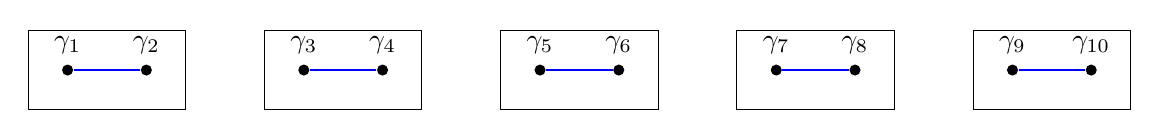
\begin{tikzpicture}[site/.style={rectangle, draw, minimum size=1cm, minimum width=2cm}]
    
    % Intra-cell pairing
    \foreach \i in {1,...,5} {
        % Calculate the labels for c
        \pgfmathtruncatemacro{\labelone}{2*\i-1}
        \pgfmathtruncatemacro{\labeltwo}{2*\i}
    
        % Draw the site
        \node[site] (site\i) at (3*\i-3,0) {};
    
        % Draw Majorana operators and labels
        \node[circle,fill=black,inner sep=0pt,minimum size=4pt,label=above:\( \gamma_{\labelone} \)] (c\labelone) at ([xshift=-0.5cm]site\i.center) {};
        \node[circle,fill=black,inner sep=0pt,minimum size=4pt,label=above:\( \gamma_{\labeltwo} \)] (c\labeltwo) at ([xshift=0.5cm]site\i.center) {};
    
        % Draw the pairing line
        \draw[thick, blue] (c\labelone) -- (c\labeltwo);
    }
    \end{tikzpicture}
    \end{center}
    los Majoranas se acoplan con los del mismo sitio. Entonces, en la fase trivial no pasa nada interesante. El estado fundamental estar\'{a} todo lleno o todo vac\'{i}o dependiendo del $\mu$, y el espectro no contiene estados de energ\'{i}a nulo.\\
(ii) Fase topol\'{o}gica. $\mu=0$ y $t=\Delta\neq 0$. Volvemos a reemplazar todos los operadores fermi\'{o}nicos por Majoranas y vemos qu\'{e} pasa
    \begin{equation}
        \begin{split}
            H&=\sum_{n=1}^N -t(c_n^\dagger c_{n+1}+c_{n+1}^\dagger c_n) + \Delta c_n c_{n+1}+\Delta^*c^\dagger_{n+1}c_n^\dagger\\
            &=\sum_{n=1}^N-\frac{t}{4}\Big[(\gamma_{2n-1}-i\gamma_{2n})(\gamma_{2n+1}+i\gamma_{2n+2})+(\gamma_{2n+1}-i\gamma_{2n+2})(\gamma_{2n-1}+i\gamma_{2n})\Big]\\
            &+\frac{\Delta}{4} (\gamma_{2n-1}+i\gamma_{2n})(\gamma_{2n+1}+i\gamma_{2n+2})+\frac{\Delta^*}{4}(\gamma_{2n+1}-i\gamma_{2n+2})(\gamma_{2n-1}-i\gamma_{2n})\\
            &=\frac{1}{4}\sum_{n=1}^N -t\Big[ \gamma_{2n-1}\gamma_{2n+1}+i\gamma_{2n-1}\gamma_{2n+2}+i\gamma_{2n}\gamma_{2n+1}\\    &+\gamma_{2n}\gamma_{2n+2}+\gamma_{2n+1}\gamma_{2n-1}+i\gamma_{2n+1}\gamma_{2n}-i\gamma_{2n+2}\gamma_{2n-1}+\gamma_{2n+2}\gamma_{2n} \Big]\\
            &+\frac{\Delta}{4}\Big[ \gamma_{2n-1}\gamma_{2n+1}+i\gamma_{2n-1}\gamma_{2n+2}+i\gamma_{2n}\gamma_{2n+1}-\gamma_{2n}\gamma_{2n+2}\\
            &+\gamma_{2n+1}\gamma_{2n-1}-i\gamma_{2n+1}\gamma_{2n}-i\gamma_{2n+2}\gamma_{2n-1}-\gamma_{2n+2}\gamma_{2n}\Big]\\
            &=\frac{t}{4}\sum_n[-2i\gamma_{2n-1}\gamma_{2n+2}+2i\gamma_{2n}\gamma_{2n+1}+2i\gamma_{2n-1}\gamma_{2n+2}+2i\gamma_{2n}\gamma_{2n+1}]\\
            &=t\sum_n i\gamma_{2n}\gamma_{2n+1}
        \end{split}
    \end{equation}
        %
    % Figura
    %
    \begin{center}
        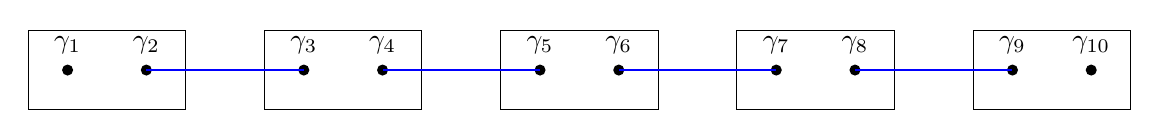
\begin{tikzpicture}[site/.style={rectangle, draw, minimum size=1cm, minimum width=2cm}]

    % Draw sites and Majorana fermions
    \foreach \i in {1,...,5} {
        % Calculate the labels for c
        \pgfmathtruncatemacro{\labelone}{2*\i-1}
        \pgfmathtruncatemacro{\labeltwo}{2*\i}
    
        % Draw the site
        \node[site] (site\i) at (3*\i-3,0) {};
    
        % Draw Majorana operators and labels
        \node[circle,fill=black,inner sep=0pt,minimum size=4pt,label=above:\( \gamma_{\labelone} \)] (c\labelone) at ([xshift=-0.5cm]site\i.center) {};
        \node[circle,fill=black,inner sep=0pt,minimum size=4pt,label=above:\( \gamma_{\labeltwo} \)] (c\labeltwo) at ([xshift=0.5cm]site\i.center) {};
    }
    
    % Draw the inter-cell pairing lines as solid lines connecting the rightmost Majorana of one site to the leftmost Majorana of the next
    \foreach \i [evaluate=\i as \nexti using int(\i+1)] in {1,...,4} {
        \pgfmathtruncatemacro{\labeltwo}{2*\i}
        \pgfmathtruncatemacro{\labelthree}{2*\i+1}
        \draw[thick, blue] ([xshift=0.5cm]site\i.center) -- ([xshift=-0.5cm]site\nexti.center);
    }
    \end{tikzpicture}
    \end{center}
    En este caso vemos que ahora los Majoranas tipo 2 de un sitio se acoplan con los de tipo 1 pero del sitio siguiente. Este acoplamiento da lugar a que los operadores de Majorana de los bordes no aparezcan en el Hamiltoniano. Por lo tanto, ambos tendr\'{i}an energ\'{i}a degenerada en cero. Adem\'{a}s, gracias a esto tenemos dos estados fundamentales degenerados ortogonales entre s\'{i}. Para ver esto definimos nuevos operadores fermi\'{o}nicos pero conformados por estos Majoranas acoplados
    \begin{equation}
        \tilde c^\dagger_j=(\gamma_{2j}-i\gamma_{2j+1})/2,\quad \tilde c_j = (\gamma_{2j}+i\gamma_{2j+1})/2
    \end{equation}
    \begin{equation}
        \gamma_{2j}=\tilde c_j^\dagger+\tilde c_j,\quad \gamma_{2j+1}=\frac{\tilde c_j^\dagger-\tilde c_j}{i}
    \end{equation}
    reemplazando en el Hamiltoniano este se convierte en
    \begin{equation}
        \begin{split}
            H&=it\sum_{n=1}^{N-1}\gamma_{2n}\gamma_{2n+1}\\
            &=it\sum_{n=1}^{N-1}\Big(\tilde c^\dagger_j - \tilde c_j \Big)\Big(\frac{\tilde c^\dagger_j + \tilde c_j}{i} \Big)\\
            &=t\sum_{n=1}^{N-1} \tilde{c_j}^\dagger\tilde{c_j}^\dagger+ \tilde{c_j}^\dagger\tilde{c_j}- \tilde c_j \tilde{c_j}^\dagger-\tilde c_j \tilde c_j\\
            &=2t\sum_{n=1}^{N-1}\Big(\tilde c_j^\dagger \tilde c_j - \frac{1}{2}\Big)
        \end{split}
        \label{hammy_kitaev_topo}
    \end{equation}
Teniendo estos dos casos a la mano podemos conjeturar que existen dos fases bien diferenciadas en el sistema dependiendo de los valores de los par\'{a}metros. Al primer caso lo llamamos el caso trivial ya que no est\'{a} pasando nada interesante y el rol de los Majorana no importa mucho. Sin embargo, en el segundo caso vemos c\'{o}mo la presencia de los Majorana de los bordes constituyen un fermi\'{o}n de Dirac deslocalizado de energ\'{i}a cero en medio del gap. Esta fase, donde hay estados con energ\'{i}as muy cercanas a cero en medio del gap, ser\'{a} llamada \emph{fase topol\'{o}gica}.
%
%
%
\section{Modelo previo de un punto cu\'{a}ntico acoplado a un cable superconductor topol\'{o}gico}
Ahora introduciremos el modelo base con el que se trabaja en la tesis: un punto cu\'{a}ntico acoplado a uno de los extremos de un nanocable. El porqu\'{e} resulta este modelo interesante es que se puede usar el punto cu\'{a}ntico como una prueba local para realizar espectroscop\'{i}a de Majoranas en un nanocable supercondutor. Esta configuraci\'{o}n nos va a permitir disernir si los modos cero que se observan en los experimentos de anomal\'{i}as de pico cero son de origen topol\'{o}gico o si se trata de alg\'{u}n otro fen\'{o}meno f\'{i}sico. Los primeros en proponer este sistema fueron Prada \emph{et alia} \cite{PhysRevB.96.085418}. En su investigaci\'{o}n usan un hamiltoniano efectivo a bajas energ\'{i}as y presentan una serie de simulaciones del perfil de espectro de energ\'{i}as donde dependiendo si se trata de un cable corto ($\approx 400$ nm) o cable largo ($\approx 2$ $\mu$m) se puede apreciar o bien diferentes patrones que forman los MZMs, como de  mo\~{n}o o diamante, o una protecci\'{o}n topol\'{o}gica muy robusta incluso si las energ\'{i}as de los autoestados correspondientes al punto cu\'{a}ntico se acercan mucho al cero, pero no tanto como para cruzarse con los MZMs. Luego, Clarke \cite{PhysRevB.96.201109}, extiende estos estudios para medir la calidad o grado de qu\'{e} tan topol\'{o}gico es un sistema de las mismas caracter\'{i}sticas que el modelo de Prada \emph{et alia}. Finalmente, Ricco \emph{et alia} \cite{PhysRevB.102.165104} hacen una extensi\'{o}n m\'{a}s a este modelo incluyendo un t\'{e}rmino de repulsi\'{o}n coulombiana afirmando que este induce una hibridaci\'{o}n adicional en los MZMs. Algunos estudios experimentales que le dan soporte a todos estos trabajos pueden ser le\'{i}dos en las referencias \cite{PhysRevB.98.085125} y \cite{DEEENG}. 
%
% Estudios de Prada et al
%
\begin{comment}
\subsection{Estudio de Prada et al.}
Uno de los mayores problemas a resolver es disernir de manera correcta si en experimentos de transporte que reportan una anomalía \emph{zero-bias}, se trata realmente de Majoranas de origen topológico o si se puede explicar por otros mecanismos.
\begin{figure}[h]
    \centering
    \includegraphics[width=0.7\textwidth]{ch2f/prada1.png}
    \caption{Configuraci\'{o}n del sistema de punto cu\'{a}ntico acoplado a un nanocable.}
    \label{fig:prada_model}
\end{figure}

En el trabajo de Prada \emph{et alia} \cite{PhysRevB.96.085418}, la configuraci\'{o}n con la que trabajan es la de tener nanocables semiconductores con superconductividad inducida por proximidad. Los autores proponen atacar el problema de detectar la calidad de los Majoranas a trav\'{e}s de una sonda local, en este caso un punto cu\'{a}ntico. Su modelo es el de tener a este en uno de los extremos del nanocable, el potencial qu\'{i}mico ser\'{a} controlado por la fuente (\emph{source}) y sumidero (\emph{drain}), la ocupaci\'{o}n del punto cu\'{a}ntico controlado por los potenciales de compuerta (\emph{gate}), e imponiendo acoplamientos $t_{L(R)}$ entre el punto cu\'{a}ntico con los Majoranas ubicados en los extremos del nanocable que llamaremos $\gamma_{L(R)}$ a izquierda y derecha, y, finalmente, incluyen un acoplamiento $\delta$ entre los Majorana tal como se ve en la figura \ref{fig:prada_model}.

Prada et alia usaron un modelo \emph{tight-binding} microsc\'{o}pico en el que corrieron simulaciones para el estudio de hibridaci\'{o}n de modos cero de Majoranas en un cable y estados de \emph{subgap} del punto cu\'{a}ntico. Su Hamiltoniano completo es
\begin{equation}
\begin{split}
H & = H_d + H_w + H_{hop}, \\
H_d & = d^{\dagger}_{\sigma'}(\epsilon_{0}\sigma_0 + B\sigma_z)d_{\sigma} + U n_{\uparrow}n_{\downarrow}, \\
H_w & = \int_{0}^{L_w} dx\text{ }c^{\dagger}_{x\sigma} \left( \frac{\hbar^2 k_x^2}{2m} - \mu \sigma_0 + \alpha k_x \sigma_y + B_0 \sigma_z \right) c_{x\sigma} \\
    & \quad + \Delta (c_{x\uparrow}c_{x\downarrow} + c^{\dagger}_{x\downarrow}c^{\dagger}_{x\uparrow}), \\
H_{hop} & = t(c^{\dagger}_{0\sigma}d_{\sigma} + d^{\dagger}_{\sigma}c_{0\sigma}),
\end{split}
\label{hammy_prada}
\end{equation}
donde $\epsilon_0$ es el nivel de energ\'{i}a del punto, $U$ es la energ\'{i}a de carga, $m$ es la masa efectiva del nanocable, $\alpha$ es el acoplamiento spin-orbita de Rashba, $\Delta$ es el apareamiento superconductor inducido, $\mu$ es el potencial qu\'{i}mico del cable, y $B$ es el desdoblamiento Zeeman original por un campo magn\'{e}tico externo. Para un $B>B_c\equiv \sqrt{\mu^2+\Delta^2}$ el nanocable entra en una fase topol\'{o}gica con estados de Majorana en cada extremo. 
\par Este es un modelo bastante general bajo ciertas reestricciones. El t\'{e}rmino de repulsi\'{o}n es local en el punto cu\'{a}ntico pero no incluye interacci\'{o}n con la cadena. El t\'{e}rmino $Un_\uparrow n_\downarrow$ lo tratan en campo medio. Por otro lado, en palabras de los autores, utilizaron el modelado m\'{a}s simple para el contacto entre el punto y la cadena dando lugar a la parte de su Hamiltoniano $H_{hop}$ que describe un posible salto entre electrones del punto y el primer sitio de la cadena con el mismo esp\'{i}n. Se\~{n}alan que una manera m\'{a}s realista de modelar lo que pasa entre entre los dos dispositivos es considerar dos segmentos del cable, simular una cierta barrera de potencial dada por una compuerta ubicada justo en la juntura donde ambos dispositivos se unen. Indican que en su modelo de \emph{tight-binding} toman una relaci\'{o}n de $1$ a $10$ entre el coeficiente de salto entre el punto cu\'{a}ntico con el extremo izquierdo de la cadena (ver figura \ref{fig:prada_model}) y el coeficiente de salto entre posiciones cercanas en la cadena. En esta tesis se sigue de manera similar tal relaci\'{o}n.
%
% Imagenes Prada y Aguado
% 
\begin{figure}[h]
    \centering
    \includegraphics[width=0.49\linewidth]{ch3f/prada1.png} 
    \caption{(a) y (c) presentan el perfil del espectro de energ\'{i}as para cuando se deja fijo un $\epsilon_0$ y se var\'{i}a el campo magn\'{e}tico. (b) y (d) presentan tambi\'{e}n espectros de energ\'{i}a pero dejando fijo $B$ y variando el nivel de energ\'{i}a del punto cu\'{a}ntico.\cite{PhysRevB.96.085418}. El tama\~{n}o del cable utilizado para sus simulaciones tiene $L_\omega=2$ $\mu$m}
    \label{fig:pradaa1}
\end{figure}

\begin{figure}[h]
    \centering
    \includegraphics[width=0.49\linewidth]{ch3f/prada2.png} 
    \caption{Espectro de energ\'{i}as para una cadena corta de longitud $L_\omega=400$ nm. (a) presenta las energ\'{i}as del sistema segun se var\'{i}a el campo magn\'{e}tico $B$, y (b) y (c) para cuando se var\'{i}a $\epsilon_0$.\cite{PhysRevB.96.085418}.}
    \label{fig:pradaa2}
\end{figure}


La fenomenolog\'{i}a de su modelo de \emph{tight-binding} es mostrada en un perfil del espectro de energ\'{i}a. En la figura \ref{fig:pradaa1}(a) y \ref{fig:pradaa1}(b) se pueden diferenciar clarmente dos fases. En la fase trivial $B<B_c$ solo los niveles del punto cu\'{a}ntico aparecen por debajo de la brecha de energ\'{i}a del superconductor. Para sus simulaciones variando el $B$, Prada \emph{et alia} consideran un nanocable de longitud $L_\omega=2$ $\mu$m con los siguientes par\'{a}metros: $\mu=0$, $\delta=0.5$ meV y un nivel energ\'{e}tico fijo del punto $\epsilon_0\approx 0.25$ meV. Para un $B>B_c$ el nanocable se encontrar\'{a} en la fase topol\'{o}gica donde podremos encontrar MZMs. Para la figura \ref{fig:pradaa2}(c) se usa un $\epsilon_0=1.0$ meV. Por otro lado, en la figura \ref{fig:pradaa2} se lidia con un nanocable corto de $\L_\omega=400$ nm. Para cables suficientemente cortos muestran que habr\'{a} una hibridizaci\'{o}n de los Majoranas que lleva a un comportamiento oscilatorio de los estados que los describen tal como vemos en la figura \ref{fig:pradaa2}(a). Cuando dejan fijo $B$ y empiezan a variar $\epsilon_0$ se observan estas mismas oscilaciones pero adoptando patrones como de mo\~{n}o o de diamante, ver figura \ref{fig:pradaa2}(b) y\ref{fig:pradaa2}(c).
\par Tambi\'{e}n ofrecen una derivaci\'{o}n de su modelo efectivo a bajas energ\'{i}as. En el trabajo original de Kitaev, este ya mencionaba que para cadenas de longitud $L$ finita habr\'{a} una interacci\'{o}n d\'{e}bil entre los dos modos cero de Majorana $\gamma_L$ y $\gamma_R$, donde $\gamma_L$ est\'{a} en el final izquierdo de la cadena y $\gamma_R$ en el final derecho. El hamiltoniano efectivo con el que Kitaev termina tiene la forma de
\begin{equation}
    H_{eff}=\frac{i}{2}t\gamma_L\gamma_R, t\propto e^{-L/l_0}.
\end{equation}
\end{comment}
%
% Estudios de ricco et al.-
%
\subsection{Estudio de Ricco \emph{et alia}}
Para esta tesis resulta importante repasar en cierto detalle el modelo planteado por Ricco \emph{et alia} ya que ser\'{a}n sus resultados los cuales compararemos con los nuestros.

El modelo de Ricco \emph{et alia} es un Hamiltoniano efectivo de bajas energ\'{i}as en el que solo est\'{a}n presentes t\'{e}rminos del punto cu\'{a}ntico y los modos fermi\'{o}nicos de Majorana que se encuentran a los extremos de la cadena unidimensional que est\'{a} acoplada en uno de los extremos con el punto cu\'{a}ntico. A esto se le a\~{n}ade el t\'{e}rmino de interacci\'{o}n coulombiana entre ambos dispositivos que, seg\'{u}n los autores, causa que el desdoblamiento de los MZMs aumente y al hacerlo estos pierden su robustez ante posibles perturbaciones. El Hamiltoniano que propusieron luce como 
\begin{equation}
    \mathcal{H}=\epsilon_d d^\dagger d + i\epsilon_M \gamma_L\gamma_R + i\lambda_L(d-d^\dagger)\gamma_L+\lambda_R(d+d^\dagger)\gamma_R + H_U
    \label{hammy_ricco}
\end{equation}
donde $\epsilon_d$ es la energ\'{i}a de ocupaci\'{o}n del punto cu\'{a}ntico, $\epsilon_M$ es una medida de qu\'{e} tanto acoplamiento o hibridizaci\'{o}n espacial existe entre las funciones de onda de los modos de Majorana de la izquierda el de la derecha, $\lambda_{L(R)}$ indica cu\'{a}nto acoplamiento hay entre los Majoranas de la izquierda y derecha respectivamente con el punto cu\'{a}ntico. Finalmente, el \'{u}ltimo t\'{e}rmino de cuenta de la repulsion coulombiana entre el punto cu\'{a}ntico y el fermi\'{o}n delocalizado $f^\dagger=(\gamma_L+\gamma_R)/2$ formado por ambos Majoranas, este posee la siguiente forma, con $n_f=f^\dagger f$
\begin{equation}
    H_U=U n_d n_f = \frac{1}{2}Un_d\Big( i\gamma_R\gamma_L+\frac{1}{2}\Big)
\end{equation}
$n_f$ representar\'{i}a el total de la ocupaci\'{o}n de la cadena a baja energ\'{i}a. $H_U$ se parece bastante a la del segundo t\'{e}rmino de (\ref{hammy_ricco}). Por eso afirman que debido a la repulsi\'{o}n coulombiana habr\'{a} una hibridizaci\'{o}n extra causando as\'{i} un desdoblamiento m\'{a}s grande en el espectro de energ\'{i}as.\\
En las siguientes subsecciones se describir\'{a}n brevemente los casos que los autores estudiaron, estos son el caso no-interactuante y el caso interactuante. Es decir, cuando tomamos o no en cuenta la repulsi\'{o}n coulombiana. Los gr\'{a}ficos que se mostrar\'{a}n acontinuaci\'{o}n son del paper original. La forma en la que calcularon su espectro de energ\'{i}a fue a trav\'{e}s del c\'{a}lculo de densidad de estados del punto cu\'{a}ntico $\rho_d(V)$ que a temperatura cero es proporcional la conductancia diferencial, $dI/dV \propto \rho_d(V)$, con $V$ correspondiendo al voltaje de bias. La densidad espectral resultante se muestra en las figuras \ref{fig:nointer} y \ref{fig:inter}.
Cabe recordar que la tesis de los autores es que debido a la repulsi\'{o}n coulombiana los MZMs perder\'{a}n su condici\'{o}n de estar topol\'{o}gicamente protegidos, y la forma de mostrarlo es a trav\'{e}s de observar qu\'{e} les pasa a estos modos en el espectro de energ\'{i}a. Si los MZMs pierden su robustez se deber\'{i}a apreciar una separaci\'{o}n de energ\'{i}a mayor donde antes no la hab\'{i}a.
%
% Non interacting case 
%
\subsubsection{Caso no interactuante}
Primero veremos el caso no interactuante, es decir, el caso en el que la repulsi\'{o}n coulombiana est\'{a} apagada. En la figura \ref{fig:nointer}(a) para cuando no hay repulsi\'{o}n y adem\'{a}s no hay separaci\'{o}n adicional por el t\'{e}rmino que acompa\~{n}a a $\epsilon_M$, nos encontramos en el caso ideal donde los MZMs est\'{a}n topol\'{o}gicamente protegidos cerca de energ\'{i}a cero. La situaci\'{o}n cambia cuando empezamos a considerar un $\epsilon_M\neq 0$, es decir, tomar en cuenta hibridaci\'{o}n entre los MZMs. Entonces los MZMs se separan en energ\'{i}a y podemos identificar figuras caracteristicas que se ven en otras referencias como la del mo\~{n}o o de diamante. En la figura \ref{fig:nointer}(b) en el caso de $\epsilon_M\gg \lambda_R$ ocurre una forma de mo\~{n}o y el cruce de nieveles en $\epsilon_d=0$. Si en cambio se considera un coeficiente de hibridaci\'{o}n de Majoranas insignificante a comparaci\'{o}n del acoplamiento entre el punto cu\'{a}ntico y el Majorana de la derecha como en la figura \ref{fig:nointer}(c), los autores obtienen una forma de diamante, o sea un desdoblamiento en $\epsilon_d=0$. Finalmente en la figura \ref{fig:nointer}(d), si los coefficientes $\epsilon_d$, $\lambda_R$ y $\lambda_L$ son comparables, se obtiene un espectro asim\'{e}trico con respecto al eje de energ\'{i}as y ocurre un desplazamiento del cruce hacia la derecha.   
%
%Inicio de Figura no interactuante
\begin{figure}[t]
    \centering
    \includegraphics[width=0.75\textwidth]{ch3f/No interactuante.png}
    \caption{Autoenergías en función de la energía del punto cuántico $\epsilon_d$ para cuando el t\'{e}rmino de repulsi\'{o}n $H_U=0$ en (\ref{hammy_ricco}).}
    \label{fig:nointer}
\end{figure}
%
% Interacting case 
%
\subsubsection{Caso interactuante}
El caso interactuante consiste en tomar en cuenta el t\'{e}rmino de repulsi\'{o}n coulombiana $Un_dn_f$, que, como se explic\'{o} anteriormente, posee una forma muy parecida a la del t\'{e}rmino de hibridaci\'{o}n de los Majorana $\epsilon_M\gamma_L\gamma_R$. Bajo este modelo y consideraciones, sus simulaciones dan que incluso en el caso $\epsilon_M=0$, como en la figura \ref{fig:inter}(a), existe una separaci\'{o}n de energ\'{i}as de los MZMs significando la p\'{e}rdida de protecci\'{o}n top\'{o}logica.

Comparando los paneles de la figura \ref{fig:inter} con los respectivos de la figura \ref{fig:nointer}, vemos que el efecto de la interacci\'{o}n $H_U$ es siempre aumentar el desdoblamiento del caso no interactuante.
%
%Inicio de figura Interactuante
\begin{figure}[t]
    \centering
    \includegraphics[width=0.74\textwidth]{ch3f/interactuante.png}
    \caption{Autoenergías en función de la energía del punto cuántico $\epsilon_d$ para cuando el t\'{e}rmino de repulsi\'{o}n $H_U\neq 0$ en (\ref{hammy_ricco}).}
    \label{fig:inter}
\end{figure}